\documentclass[a4paper,11pt]{article}
\usepackage[verbose,a4paper,tmargin=2cm,bmargin=2cm,lmargin=2.5cm,rmargin=2.5cm]{geometry}
\usepackage[utf8]{inputenc}
\usepackage{polski}
\usepackage{amsmath}
\usepackage{amsfonts}
\usepackage{amssymb}
\usepackage{lastpage}
\usepackage{indentfirst}
\usepackage{verbatim}
\usepackage{graphicx}
\usepackage{fancyhdr}
\usepackage{listings}
\usepackage{hyperref} 
\usepackage{xcolor}
\usepackage{tikz}
\usepackage{float}
\hypersetup{pdfstartview=}
\frenchspacing
\pagestyle{fancyplain}
\fancyhf{}

\usepackage{setspace}

\renewcommand{\headrulewidth}{0pt}
\renewcommand{\footrulewidth}{0.4pt}
\newcommand{\degree}{\ensuremath{^{\circ}}} 
\fancyfoot[L]{E-Biznes: Zbigniew Nowacki, Karol Podlewski, Patrycja Szczakowska}
\fancyfoot[R]{\thepage\ / \pageref{LastPage}}


\begin{document}

\begin{titlepage}
\begin{center}
\begin{tabular}{rcl}
\begin{tabular}{|r|}
\hline \\
\large{\underline{234102~~~~~~~~~~~~~~~~~~~~~~~} }\\
\small{\textit{Numer indeksu}}\\
\large{\underline{Zbigniew Nowacki~~~~~~~~} }\\
\small{\textit{Imię i nazwisko}}\\\\ \hline
\end{tabular} 
&
\begin{tabular}{|r|}
\hline \\
\large{\underline{234106~~~~~~~~~~~~~~~~~~~~~~~} }\\
\small{\textit{Numer indeksu}}\\
\large{\underline{Karol Podlewski~~~~~~~~~~~} }\\
\small{\textit{Imię i nazwisko}}\\\\ \hline
\end{tabular} 
&
\begin{tabular}{|r|}
\hline \\
\large{\underline{234121~~~~~~~~~~~~~~~~~~~~~~~} }\\
\small{\textit{Numer indeksu}}\\
\large{\underline{Patrycja Szczakowska~~~~} }\\
\small{\textit{Imię i nazwisko}}\\\\ \hline
\end{tabular} 

\end{tabular}
~\\~\\~\\ 
\end{center}
\begin{tabular}{ll}
\LARGE{\textbf{Kierunek}}& \LARGE{Informatyka Stosowana} \\
\LARGE{\textbf{Stopień}}& \LARGE{II} \\
\LARGE{\textbf{Specjalizacja}}& \LARGE{Data Science} \\
\LARGE{\textbf{Semestr}}& \LARGE{1} \\\\
\LARGE{\textbf{Data oddania}}& \LARGE{18 czerwca 2020} \\\\\\\\\\\\\\
\end{tabular}

\begin{center}
\textbf{\huge{E-Biznes}}
\textbf{\LARGE{\\Etap 3: Dokumentacja systemu}}
\textbf{\Huge{\\~\\~\\System rezerwacji\\obiektów sportowych\\~\\ JASTRZĘBIK}} 
\end{center}

\end{titlepage}

\setcounter{page}{2}
\setstretch{1.4}

\tableofcontents
\setstretch{1.2}
\newpage

%%%%%%%%%%%%%%%%%%%%%%%%%%%%%%%%%%%%%%%%%%%%%%%%%%%%%%%%%%%%%%%%%%%%%%%%

\section{Wdrożenie oraz inizjalizacja systemu}
    Usługa składa się z aplikacji klienckiej na przeglądarkę oraz aplikacji serwerowej.
    
    \begin{itemize}
        \item Backend został wykonany na platformie Java 8 z wykorzystaniem bazy H2. % docker
        \item Frontend powstał przy użyciu frameworka React.
    \end{itemize}
    
    W celu uruchomienia całego systemu należy:
    
    \begin{itemize}
        \item Skompilować i uruchomić aplikację serwerową - można to zrobić wykorzystując IDE przeznaczone do pracowania z Javą, na przykład IntelliJ IDEA, tworząc konfigurację przeznaczoną do uruchomienia aplikacji. 
        \item Skompilować i uruchomić aplikację kliencką - konieczny do tego będzie menadżer pakietów dla środowiska Node.js - npm. Znajdując się w folderze z aplikacją należy wpisać komendy:
        \begin{verbatim}
        npm install
        npm start
        \end{verbatim}
    \end{itemize}

    Po uruchomieniu każdej z aplikacji możemy już korzystać z systemu. W domyślnej przeglądarce otworzy nam się strona pod adresem \verb|localhost:3000/|.

%%%%%%%%%%%%%%%%%%%%%%%%%%%%%%%%%%%%%%%%%%%%%%%%%%%%%%%%%%%%%%%%%%%%%%%%

\newpage
\section{Dokumentacja użytkownika}

    \subsection{Strona główna}
    
    Wchodząc na stronę główną zastaniemy następujący widok:
    
    \begin{figure}[H] 
    	\begin{center}
    		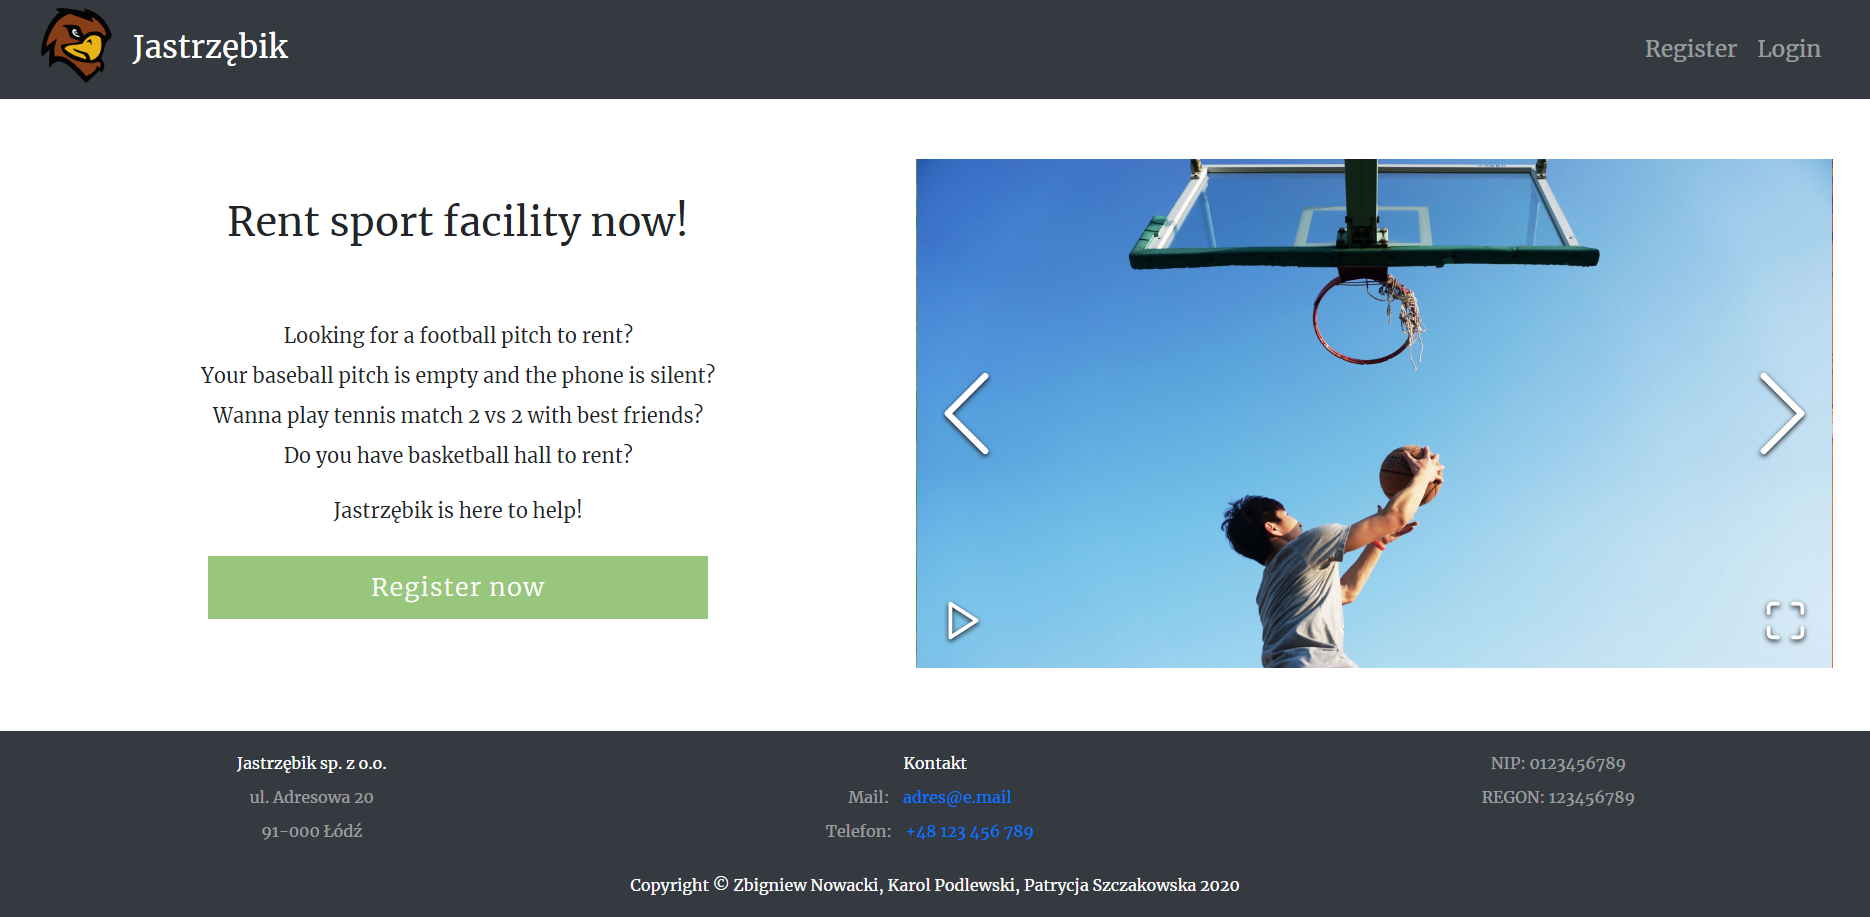
\includegraphics[width=1\textwidth]{img3/Home.png}
            \caption{Strona główna}
    	\end{center}
    \end{figure}
        
    Strona w nagłówku posiada linki przekierowujące na strony rejestracji oraz logowania, a w stopce wszystkie niezbędne informacje kontaktowe. 

    \subsection{Rejestracja i logowanie}
    
    W celu utworzenia kont użytkownika oraz animatora należy skorzystać z panelu rejestracyjnego (Rysunek \ref{fig:Reg}).
    
    \begin{figure}[H] 
    	\begin{center}
    		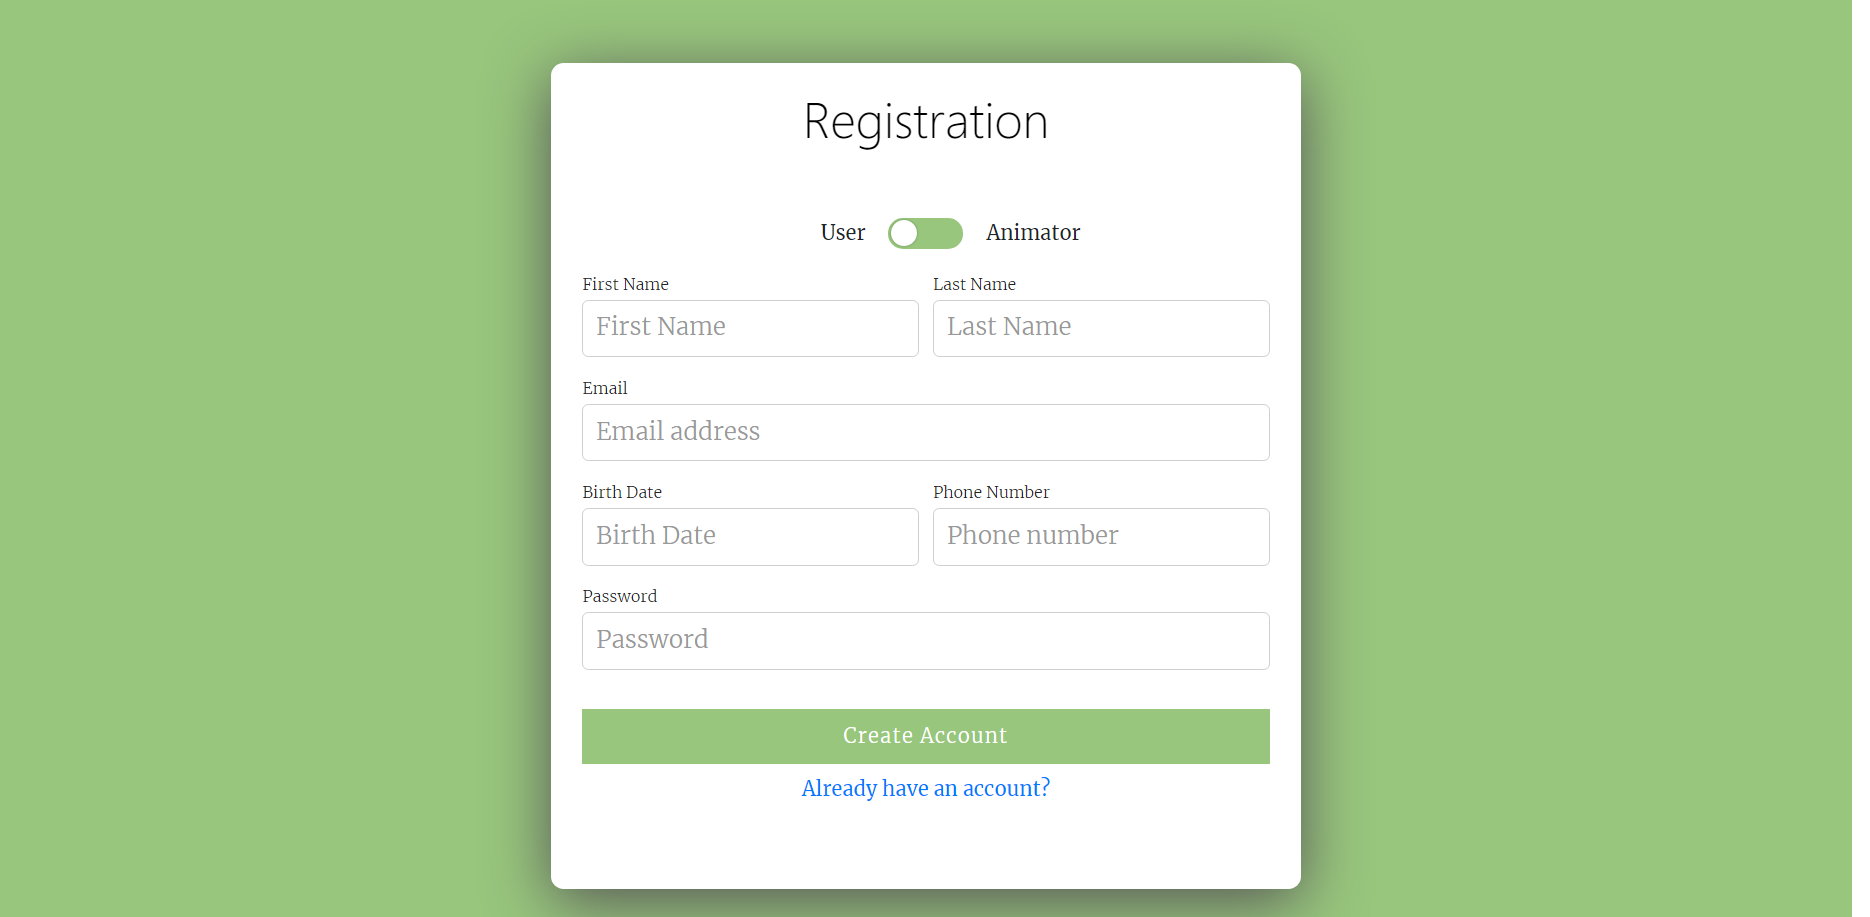
\includegraphics[width=1\textwidth]{img3/Register.png}
            \caption{Rejestracja w systemie}
            \label{fig:Reg}
    	\end{center}
    \end{figure}
    
    W przypadku kiedy uda nam się utworzyć konto, bądź już je posiadamy, możemy się udać na stronę logowania (Rysunek \ref{fig:Log}).
    
    \begin{figure}[H] 
    	\begin{center}
    		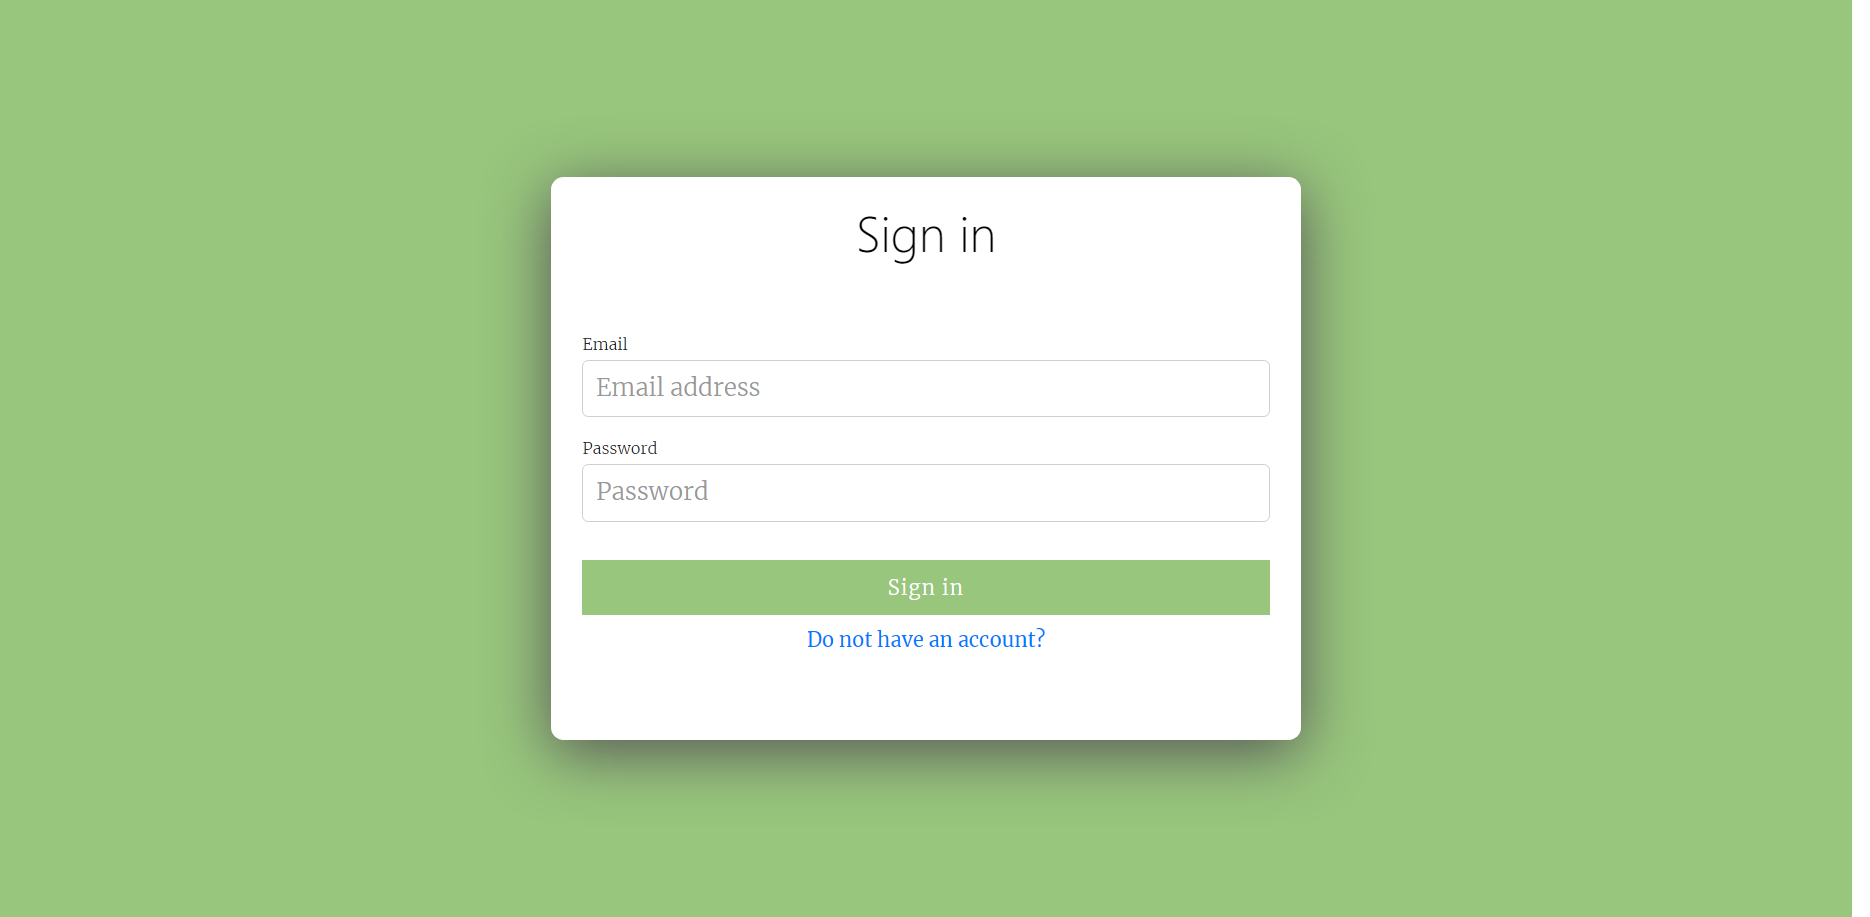
\includegraphics[width=1\textwidth]{img3/Login.png}
            \caption{Logowanie w systemie}
            \label{fig:Log}
    	\end{center}
    \end{figure}
    
    \subsection{Użytkownik zalogowany}
    
    Niezależnie od typu użytkownika, po zalogowaniu zostanie on przeniesiony na wyszukiwarkę obiektów (Rysunek \ref{fig:Search}). Umożliwia ona wyszukiwanie obiektów po nazwie, a także odfiltrowanie po miastach.
    
    \begin{figure}[H] 
    	\begin{center}
    		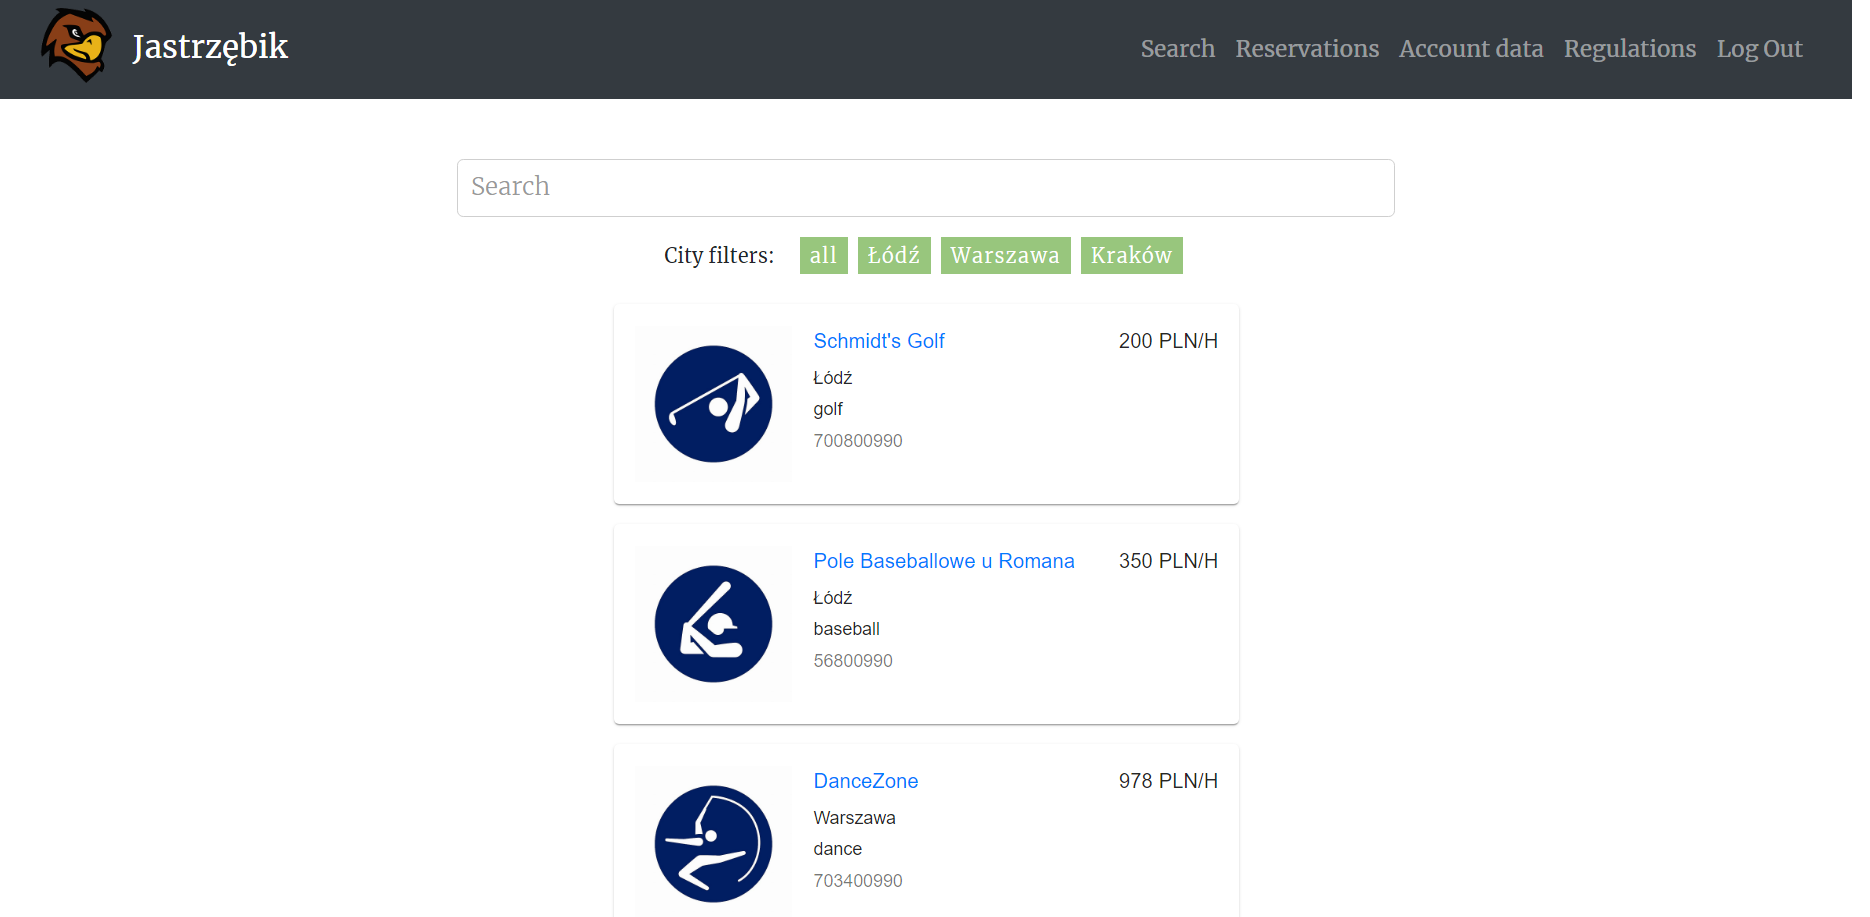
\includegraphics[width=1\textwidth]{img3/Search.png}
            \caption{Panel przeszukiwania z widocznym paskiem nawigacyjnym zwykłego użytkownika}
            \label{fig:Search}
    	\end{center}
    \end{figure}    
    
    Każdy może też zmienić swoje dane korzystając ze specjalnego panelu (Rysunek \ref{fig:Data}). Można też tutaj usunąć swoje konto.
    
    \begin{figure}[H] 
    	\begin{center}
    		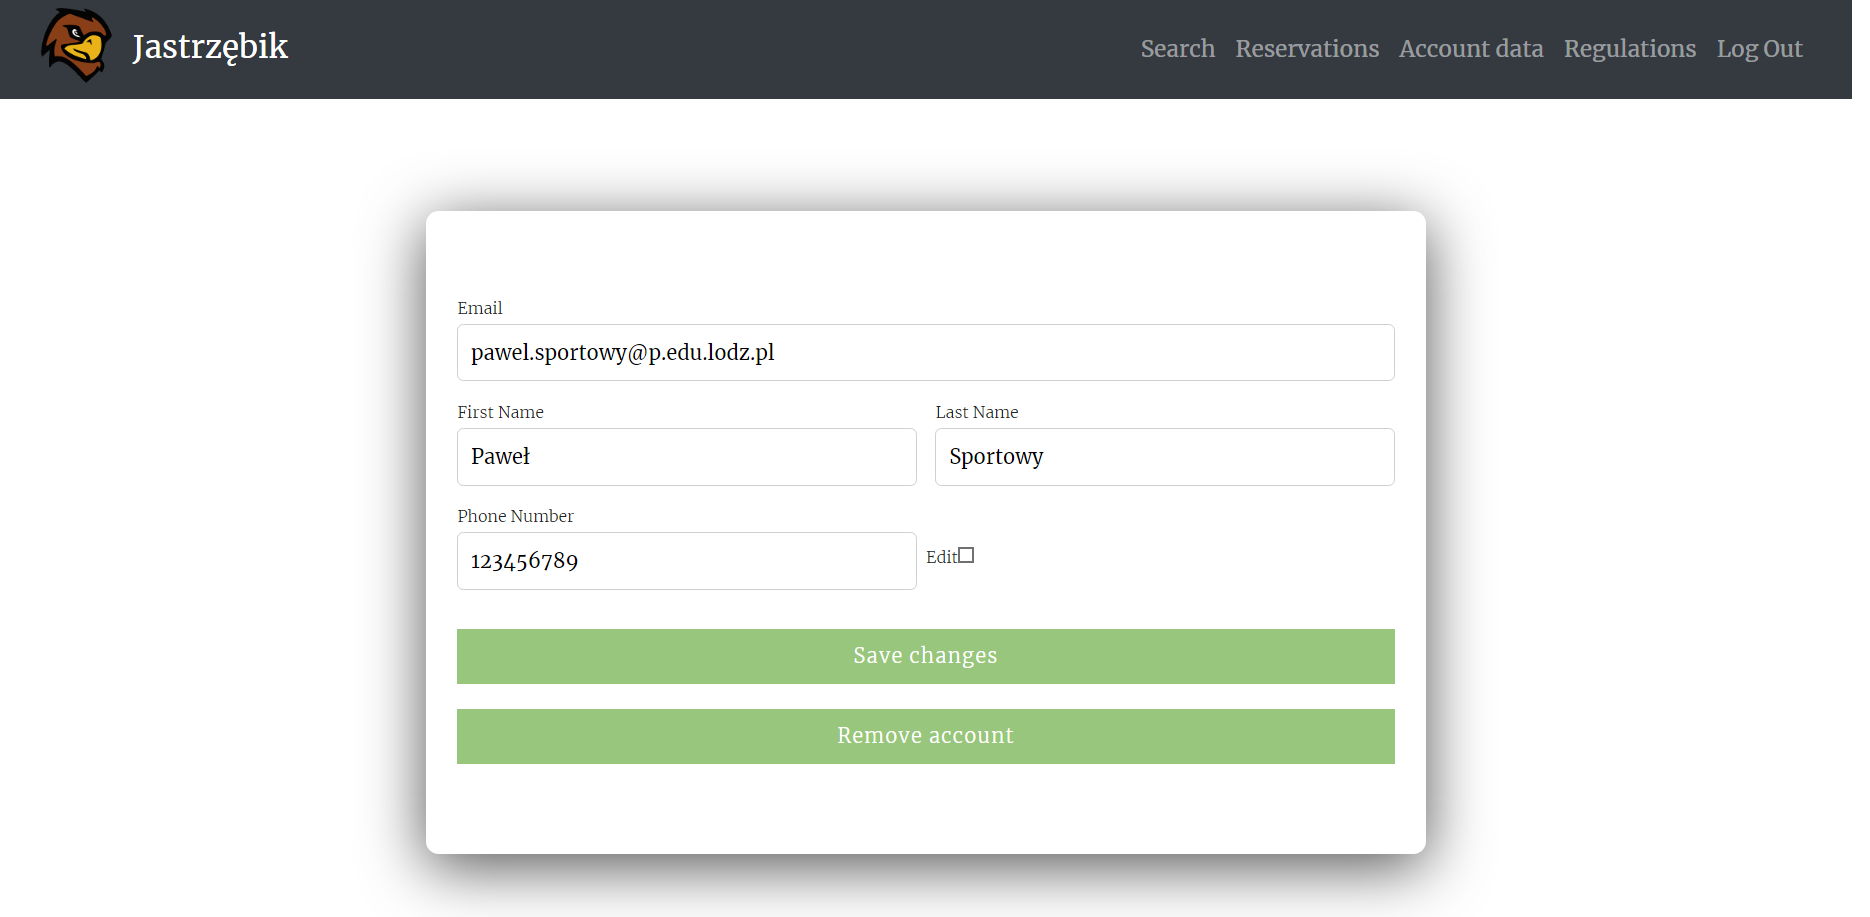
\includegraphics[width=1\textwidth]{img3/AccData.png}
            \caption{Panel zmiany danych z widocznym paskiem nawigacyjnym zwykłego użytkownika}
            \label{fig:Data}
    	\end{center}
    \end{figure}      
    
    Zalogowany użytkownik może też podejrzeć regulaminy, które są dostępne w formie do pobrania (Rysunek \ref{fig:Reg}).
        
    \begin{figure}[H] 
    	\begin{center}
    		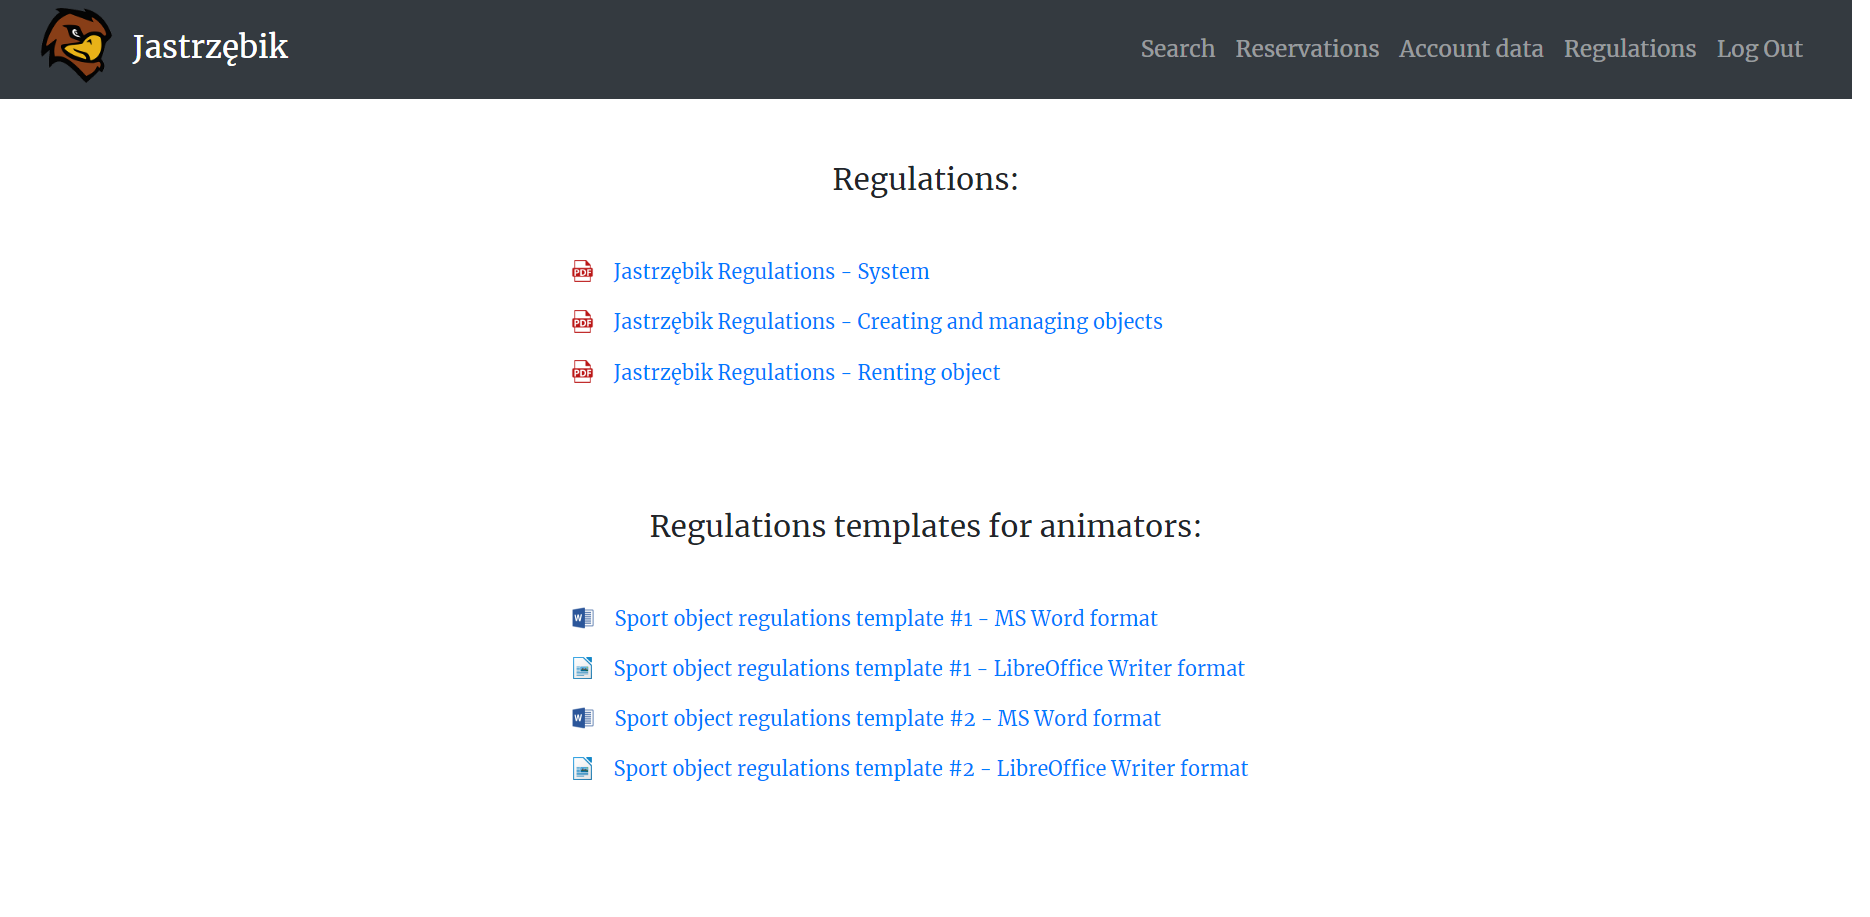
\includegraphics[width=1\textwidth]{img3/Regulations.png}
            \caption{Strona z regulaminami serwisu oraz szablonami dla regulaminów obiektów}
            \label{fig:Data}
    	\end{center}
    \end{figure}   
    
    
    \subsection{Zwykły użytkownik}

    Użytkownik może dokonywać rejestracji. Wchodząc na stronę wybranego przez siebie obiektu (Rysunki \ref{fig:Obj} oraz \ref{fig:Res}).
    
    \begin{figure}[H] 
    	\begin{center}
    		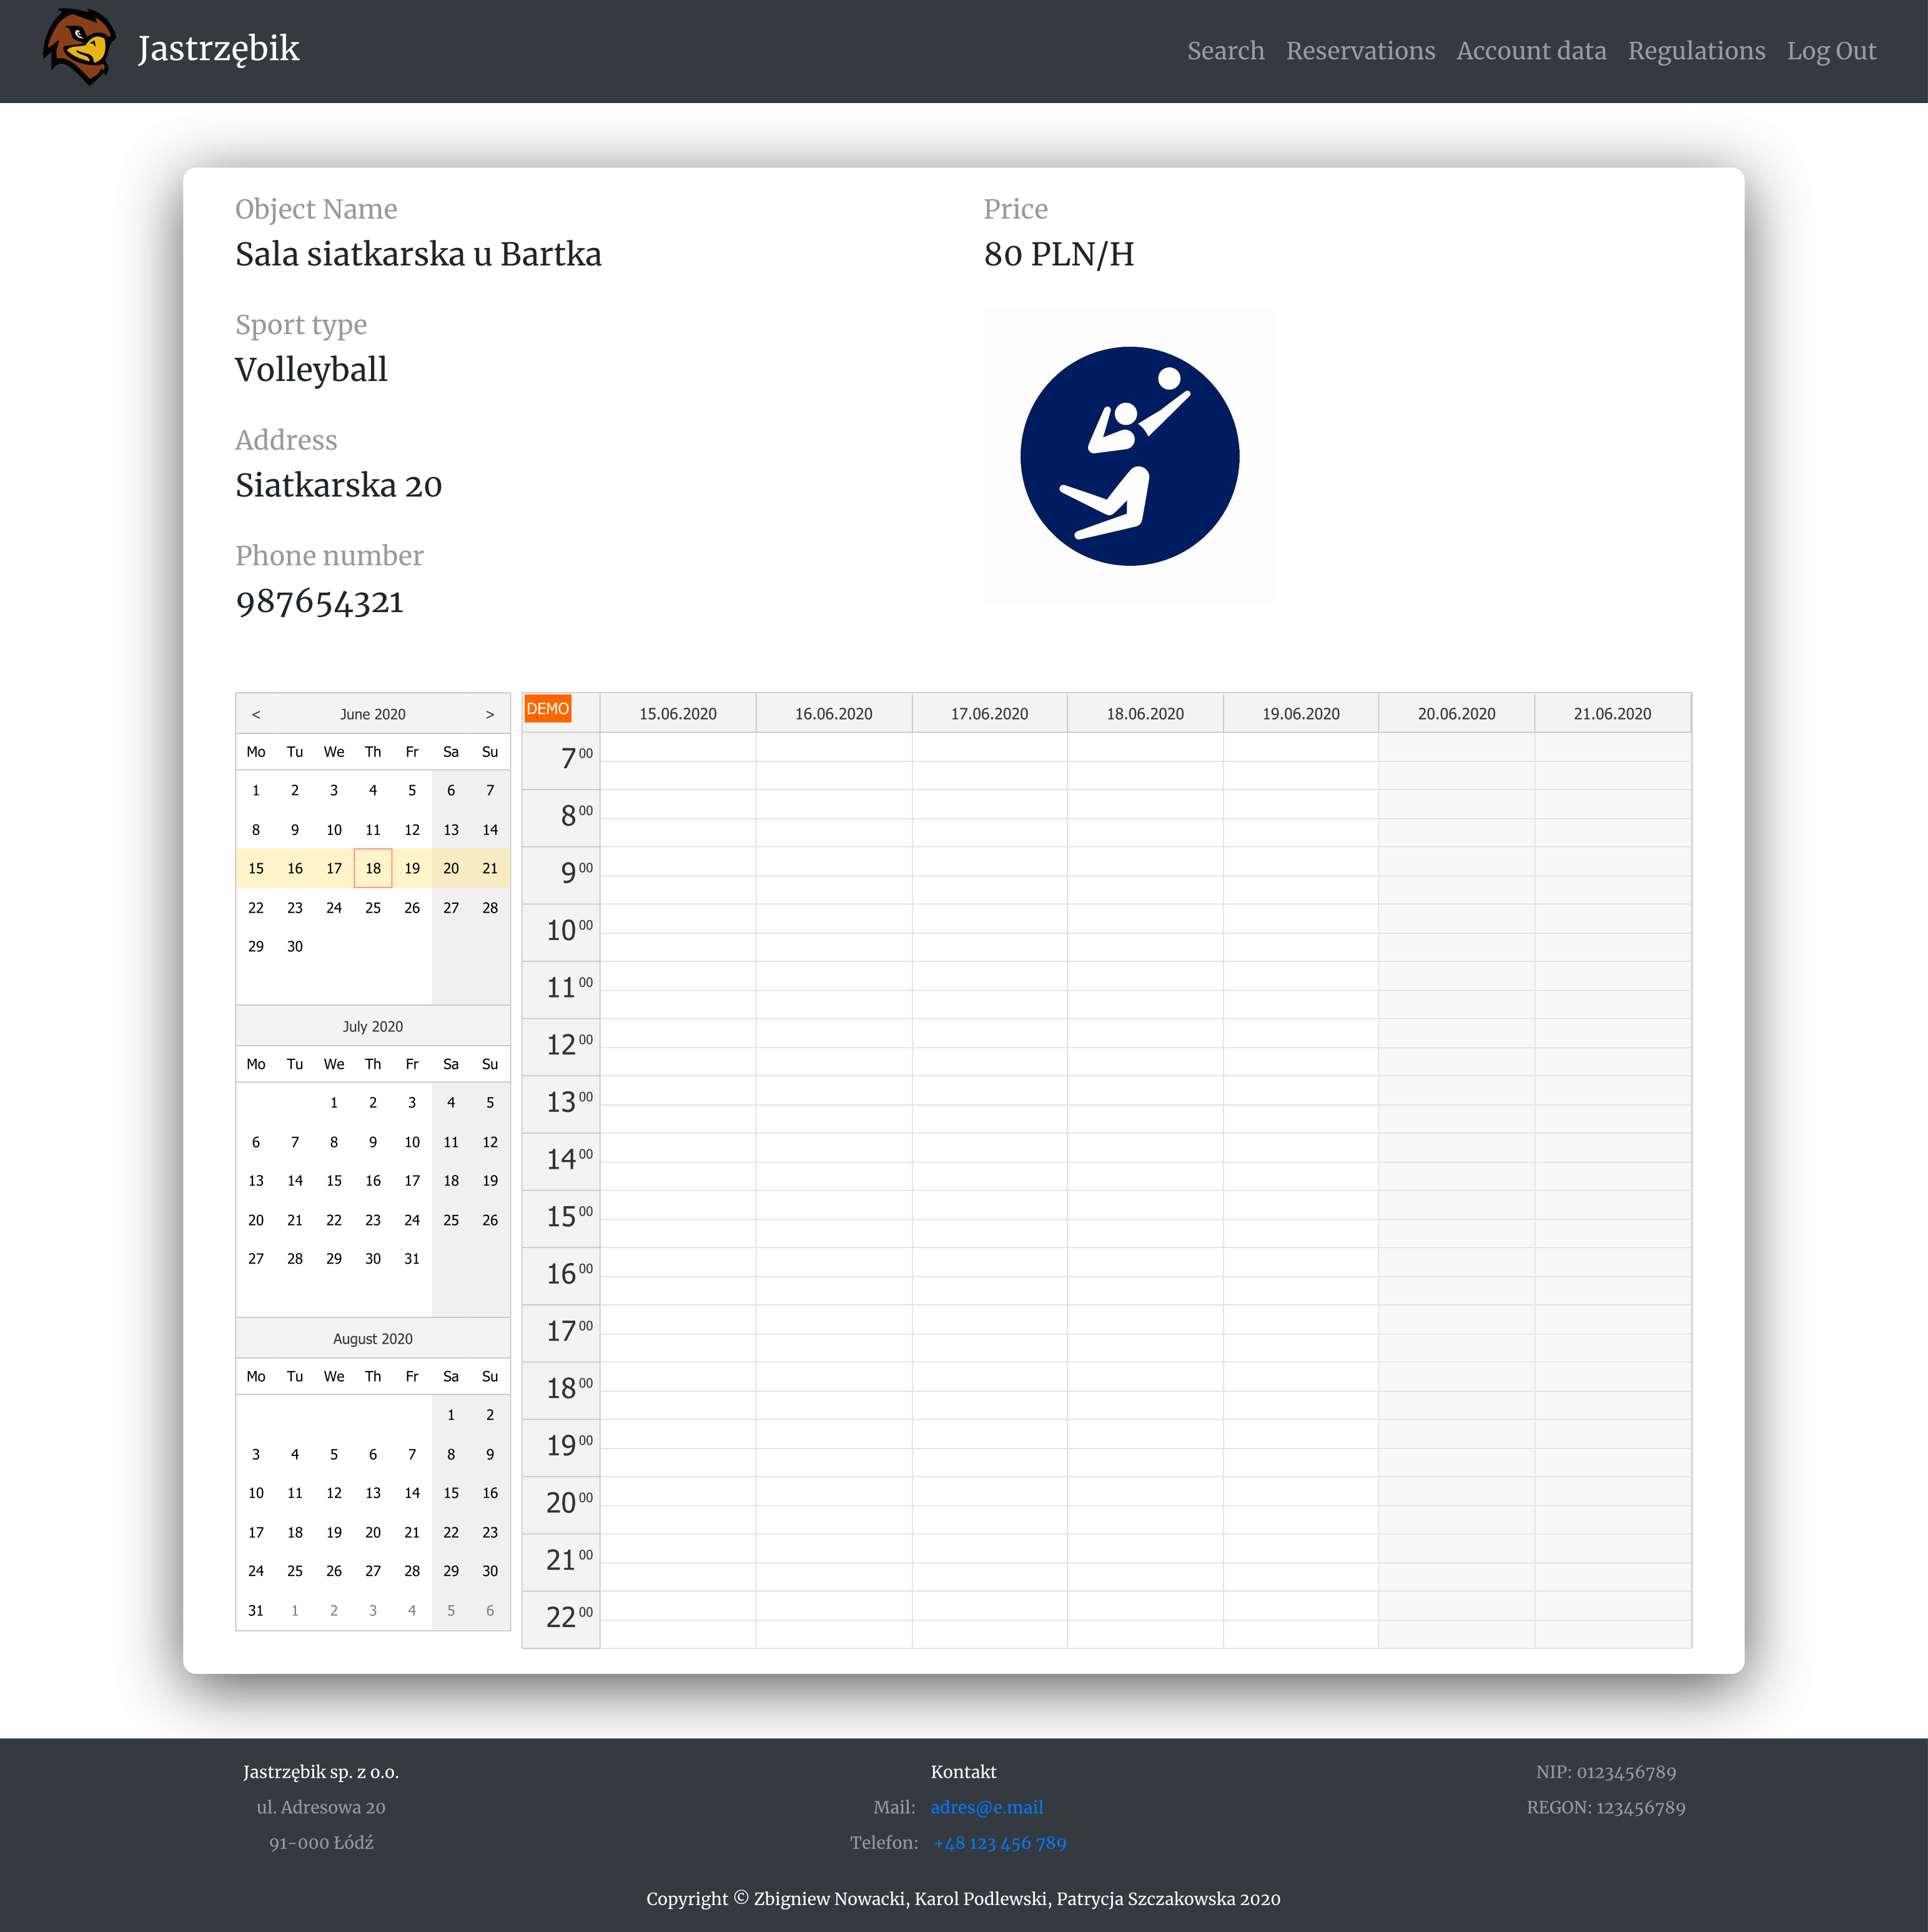
\includegraphics[width=1\textwidth]{img3/ObjPage.png}
            \caption{Podgląd wybranego obiektu}
            \label{fig:Obj}
    	\end{center}
    \end{figure}
    
    \begin{figure}[H] 
    	\begin{center}
    		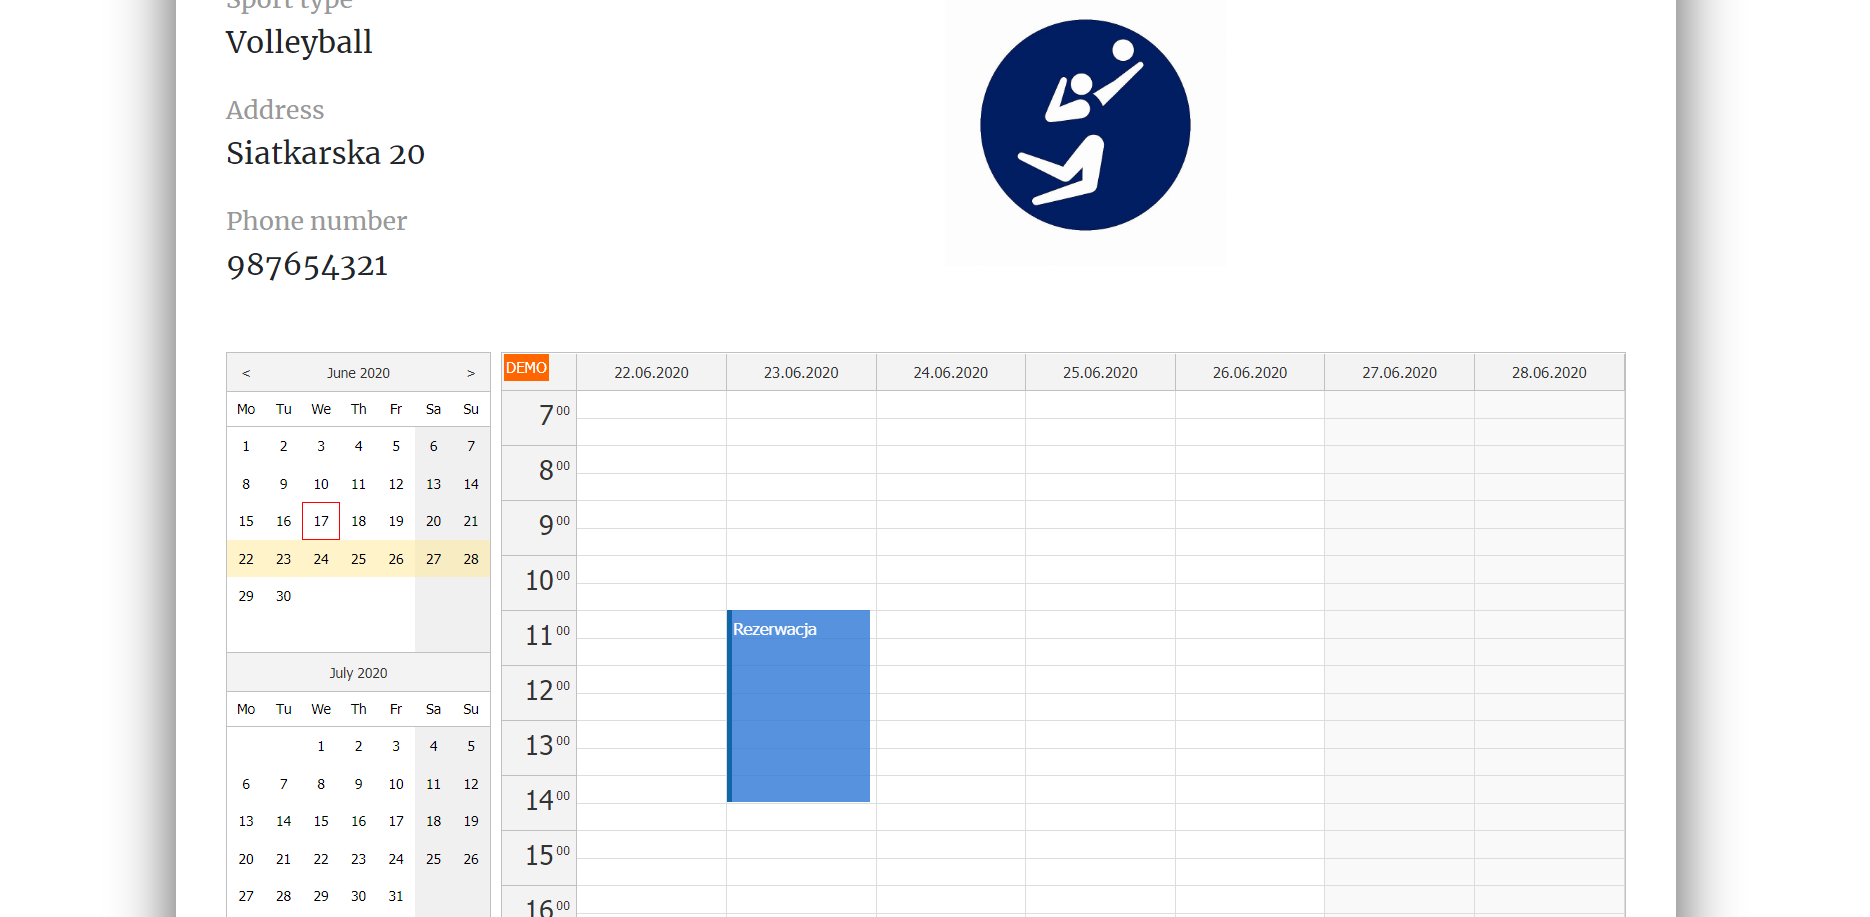
\includegraphics[width=1\textwidth]{img3/Reservation.png}
            \caption{Przykładowa rezerwacja}
            \label{fig:Res}
    	\end{center}
    \end{figure}  

    Wchodząc w panel rezerwacji, możemy ją następnie opłacić (Rysunek \ref{fig:Res2}).
    
    \begin{figure}[H] 
    	\begin{center}
    		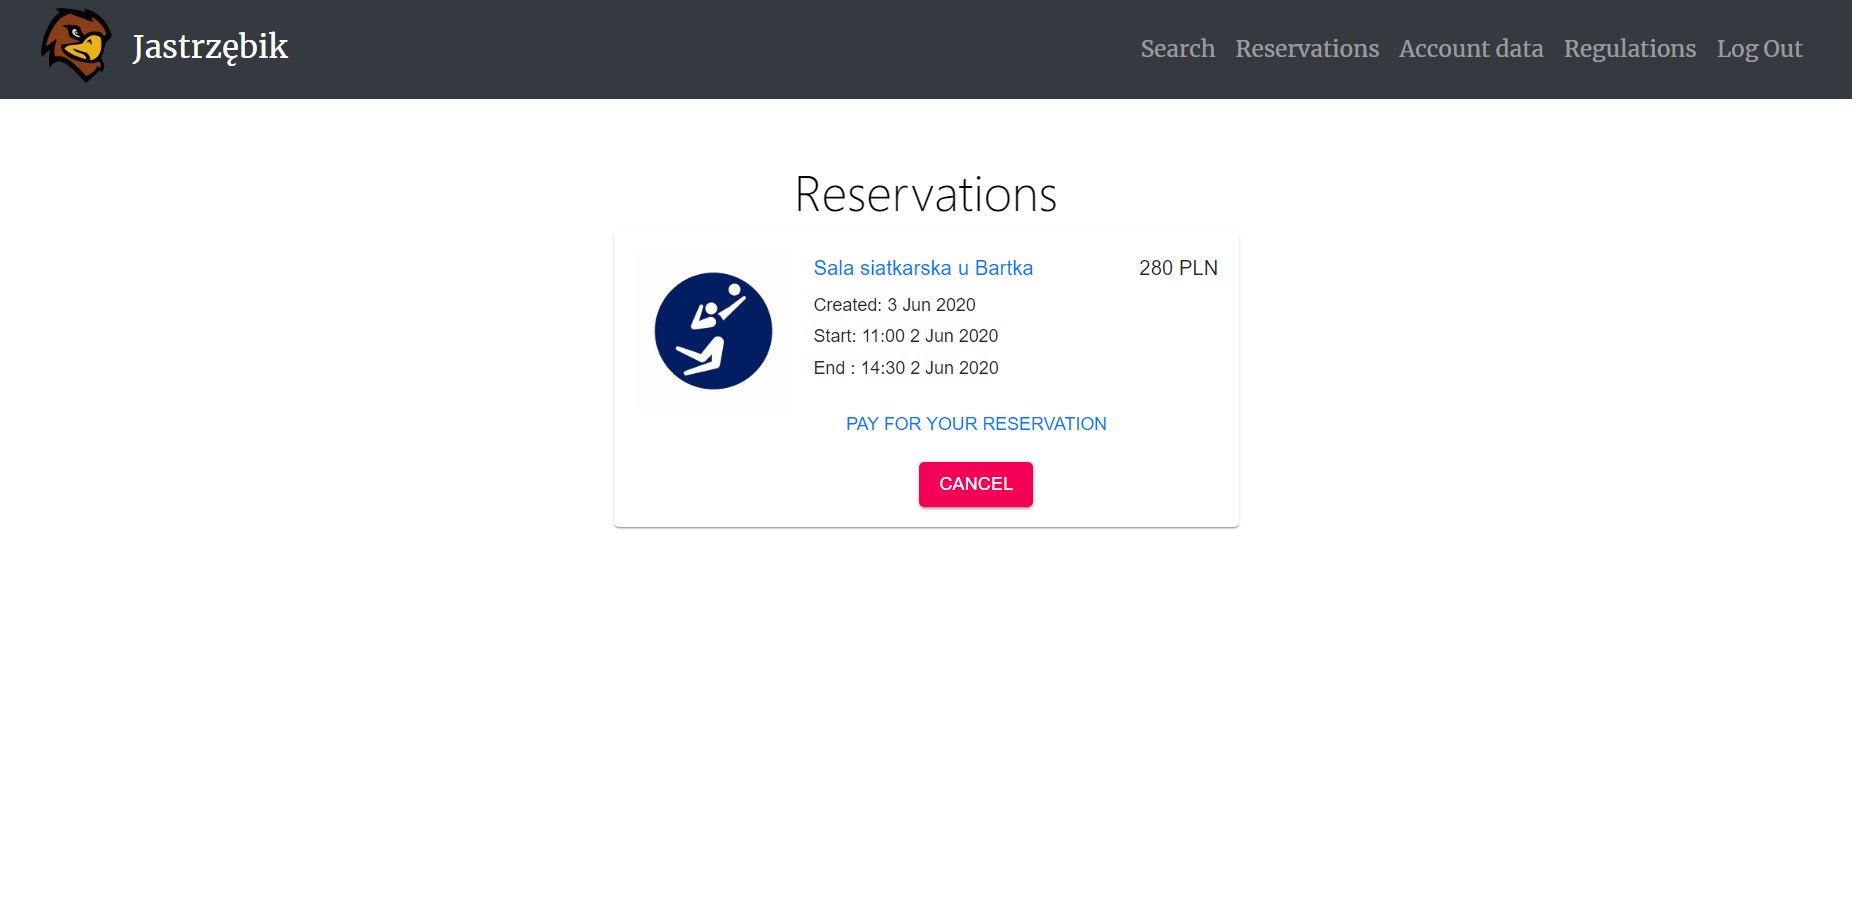
\includegraphics[width=1\textwidth]{img3/Reservations.png}
            \caption{Lista naszych rezerwacji}
            \label{fig:Res2}
    	\end{center}
    \end{figure}  
    
    W przypadku anulowanej rezerwacji, użytkownik zobaczy to na swojej liście (Rysunek \ref{fig:CancelUser}).
        
    \begin{figure}[H] 
    	\begin{center}
    		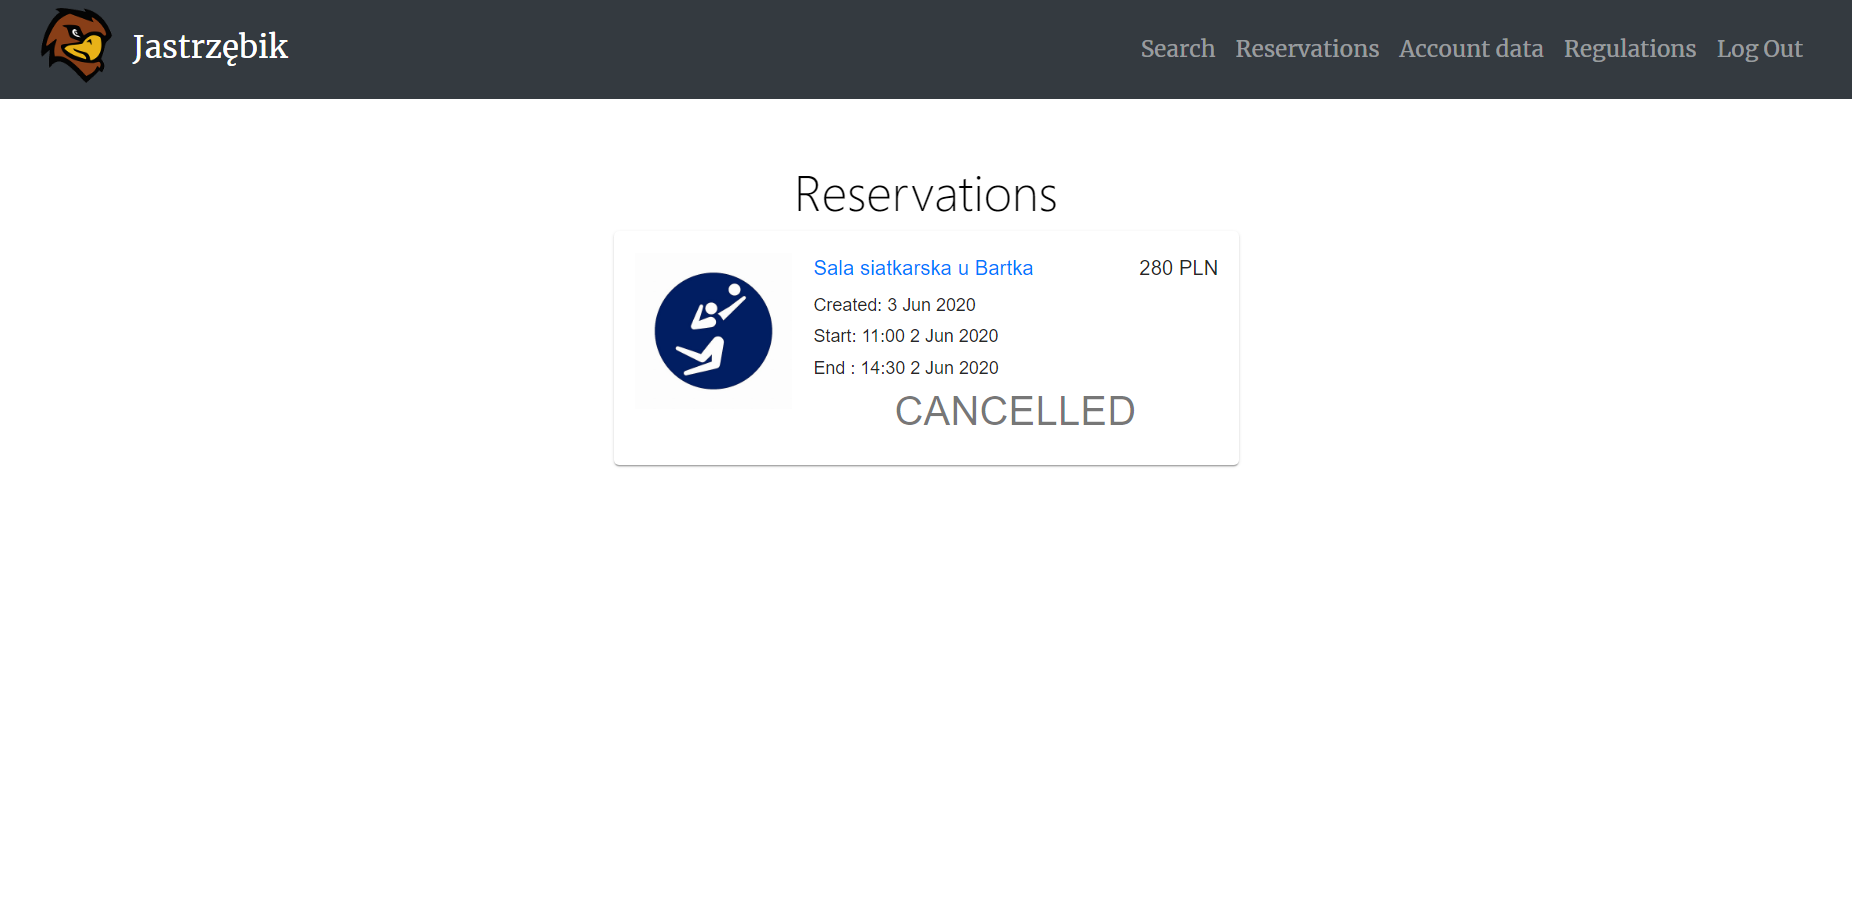
\includegraphics[width=1\textwidth]{img3/CancelUser.png}
            \caption{Przykładowa usunięta rezerwacja}
            \label{fig:CancelUser}
    	\end{center}
    \end{figure}  
    
    \subsection{Animator}
    
    Główna różnica w systemie, do którego zalogowany jest animator, to możliwość tworzenia obiektów. Animator może stworzyć nowy obiekt sportowy (Rysunek \ref{fig:CreateObj}), a także podejrzeć własne obiekty (Rysunek \ref{fig:OwnObj}). 
 
    \begin{figure}[H] 
    	\begin{center}
    		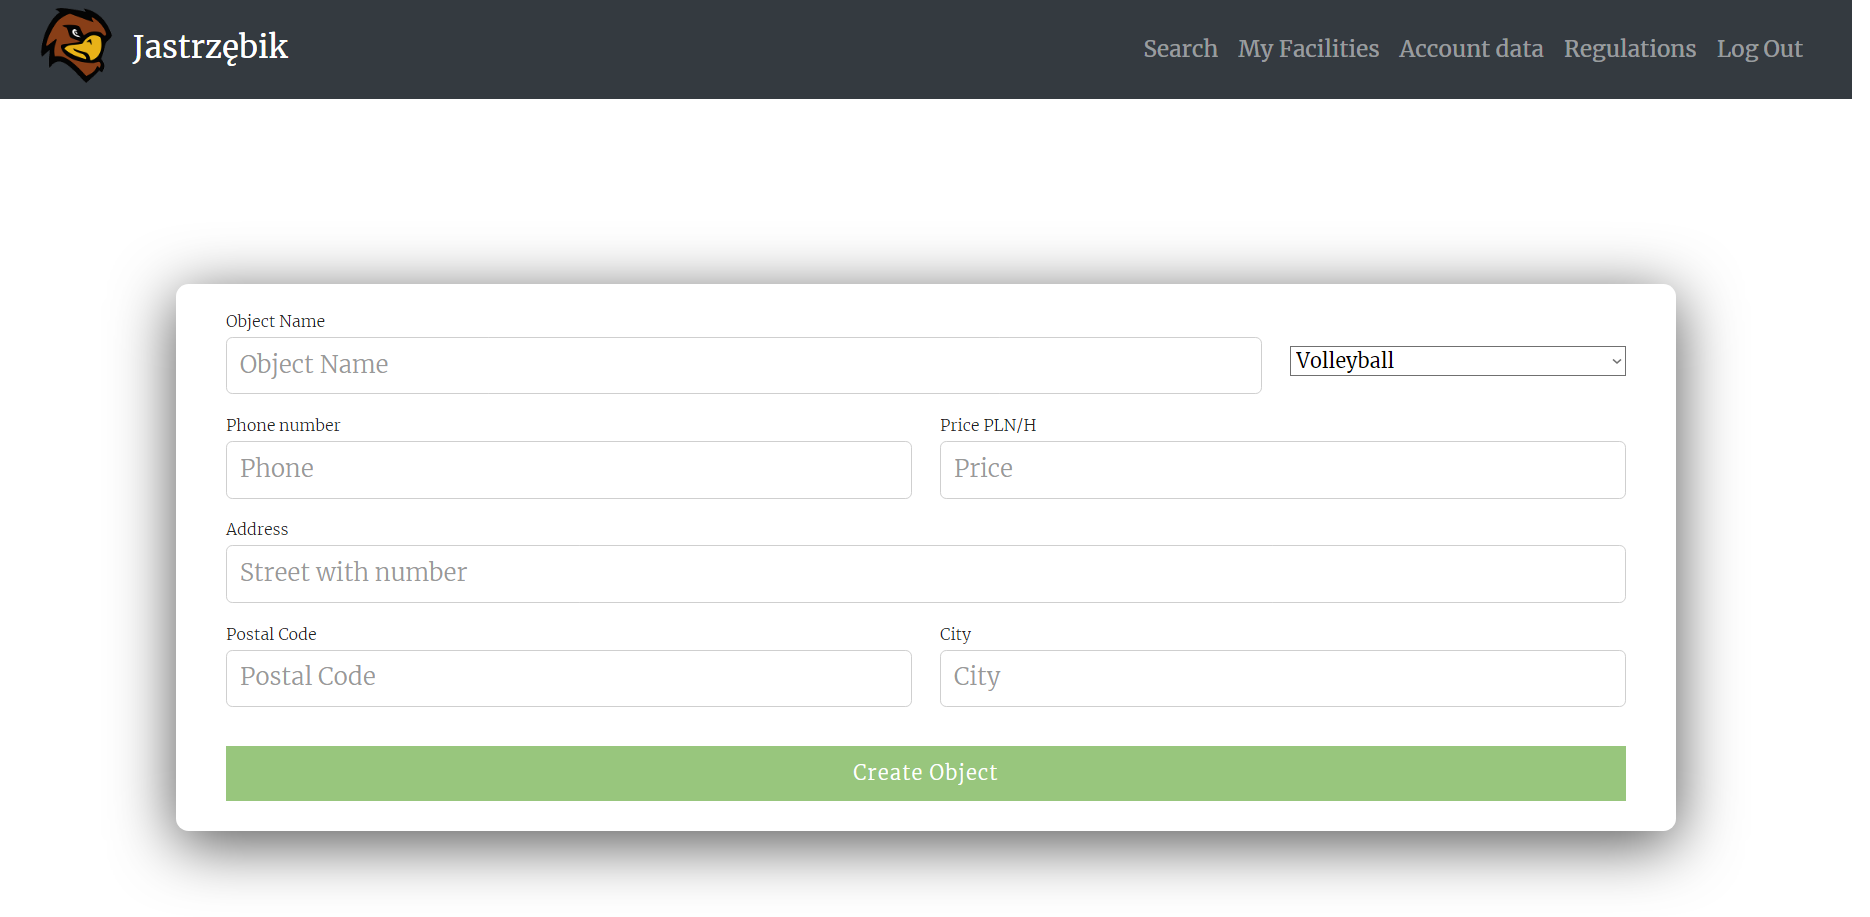
\includegraphics[width=1\textwidth]{img3/CreateObj.png}
            \caption{Panel umożliwiający tworzenie nowego obiektu sportowego}
            \label{fig:CreateObj}
    	\end{center}
    \end{figure} 
    
    \begin{figure}[H] 
    	\begin{center}
    		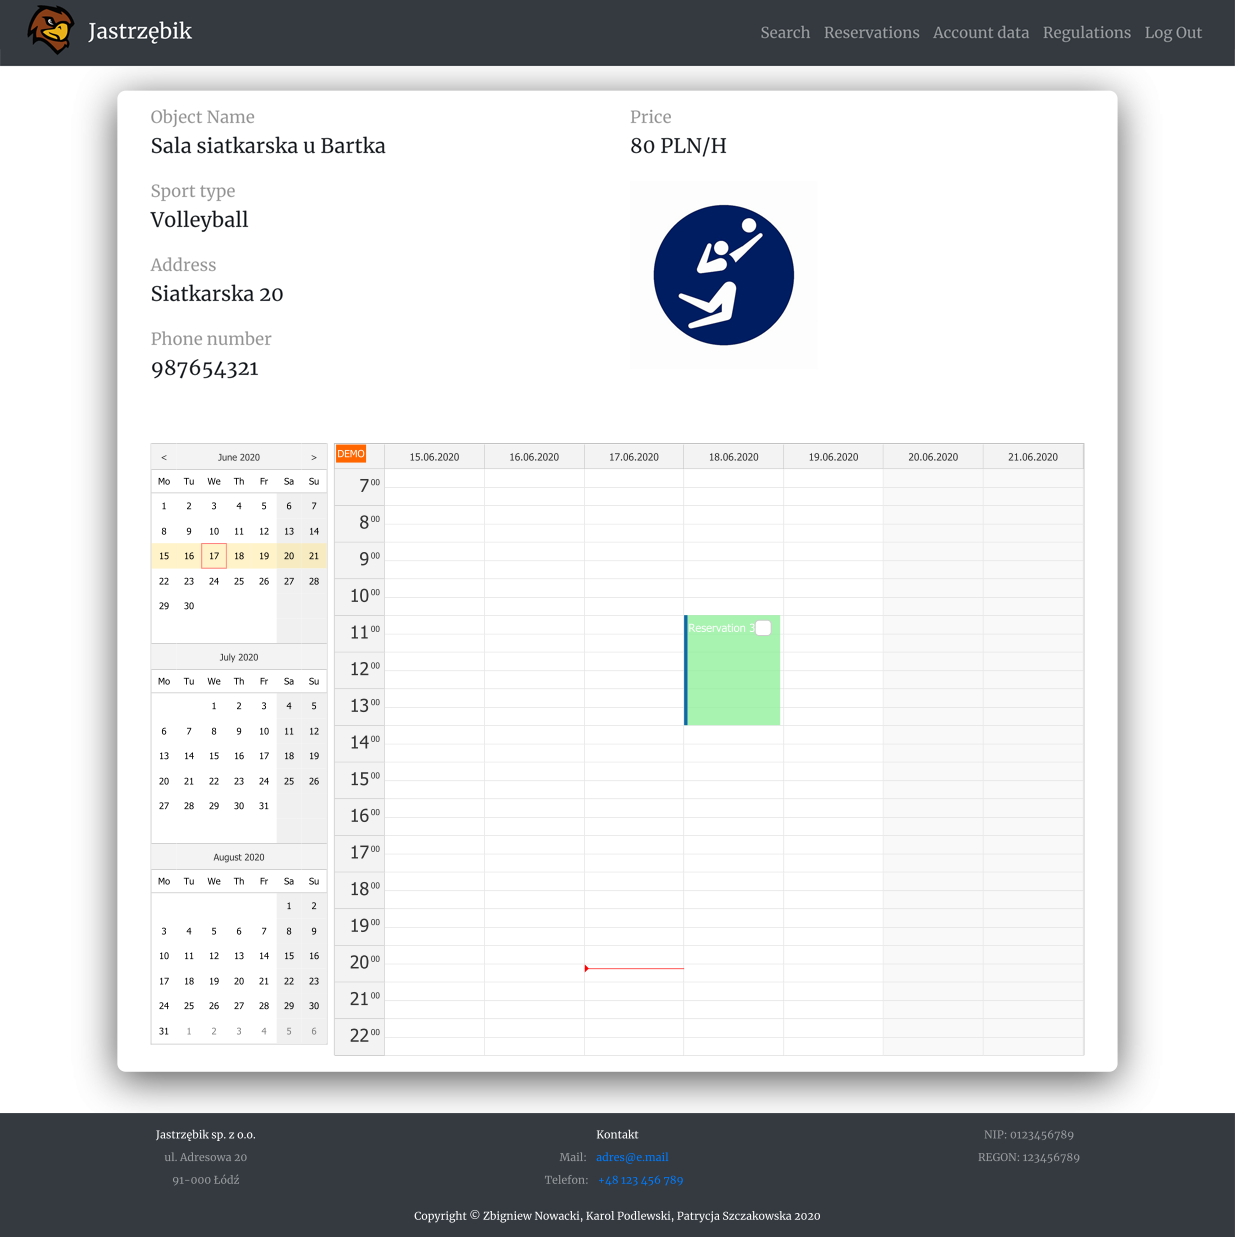
\includegraphics[width=1\textwidth]{img3/AnimObj.png}
            \caption{Podgląd własnych obiektów sportowych}
            \label{fig:OwnObj}
    	\end{center}
    \end{figure}      

    Animator może też anulować rezerwację (Rysunek \ref{fig:Can}).
        
    \begin{figure}[H] 
    	\begin{center}
    		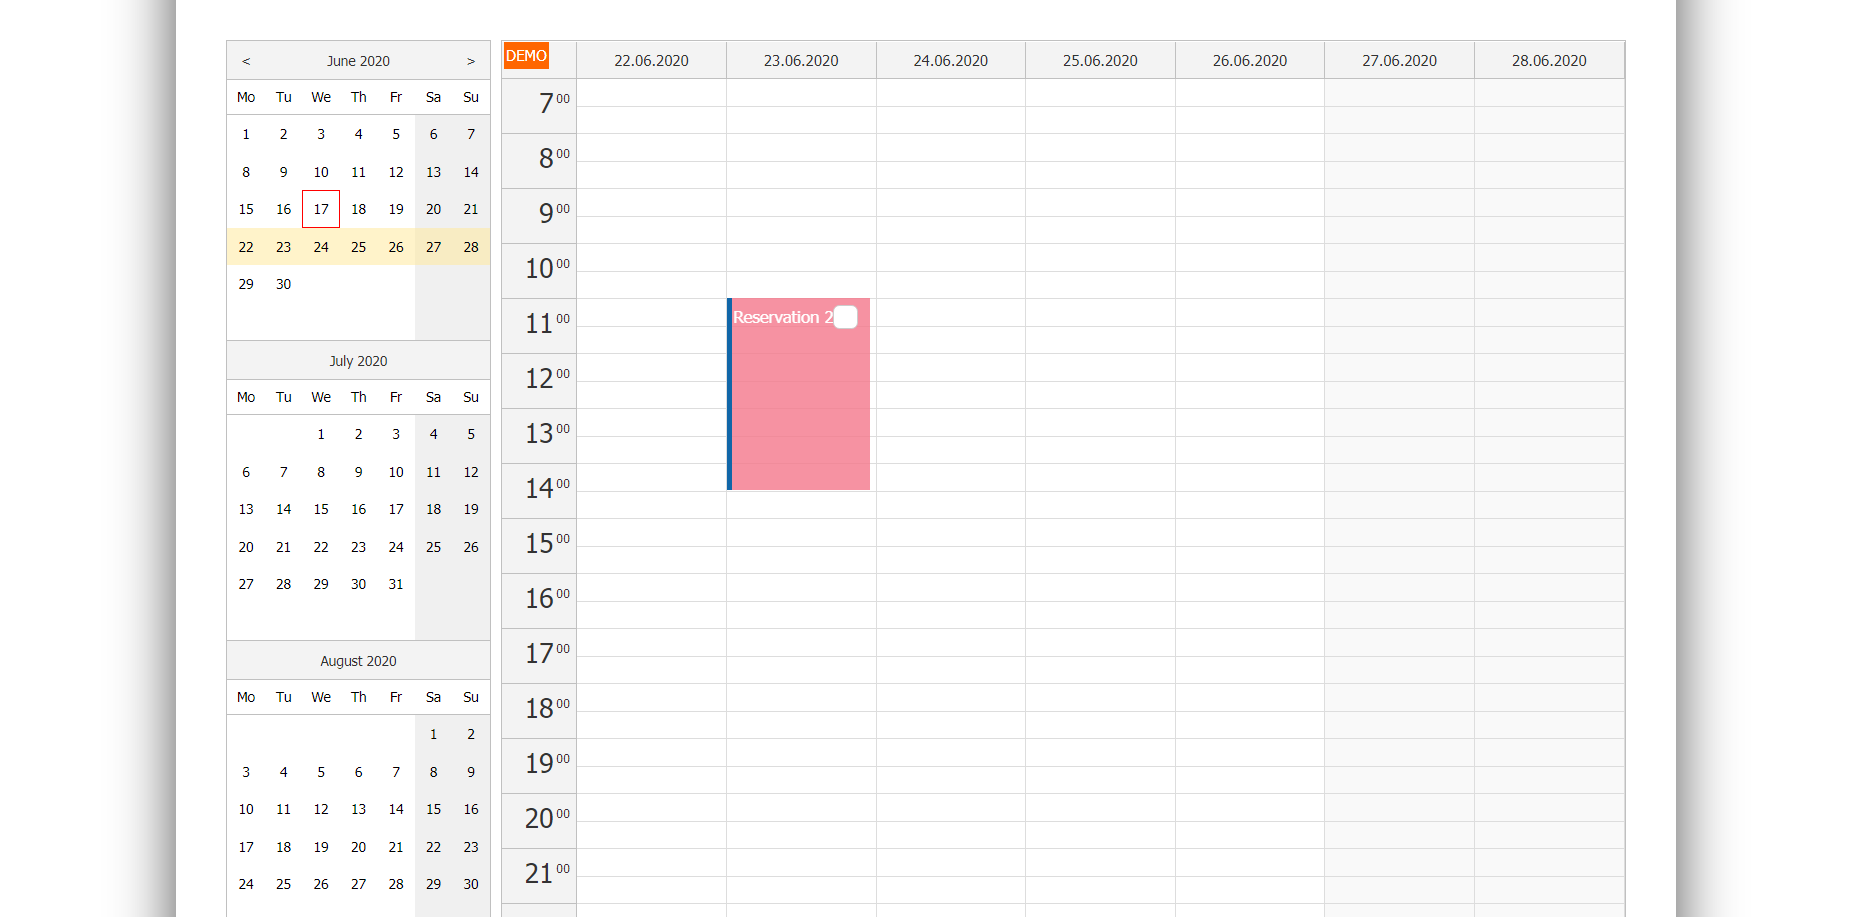
\includegraphics[width=1\textwidth]{img3/Canceled.png}
            \caption{Panel umożliwiający tworzenie nowego obiektu sportowego}
            \label{fig:Can}
    	\end{center}
    \end{figure}      

    \subsection{Administrator}
    
    Użytkownik systemu o statusie Administratora ma do dyspozycji widok z przeglądem zgłoszeń użytkowników (Rysunek \ref{fig:Reports}). Każdy wpis składa się z identyfikatorów użytkowników zgłaszającego i zgłaszanego oraz wiadomością dotyczącą zgłoszenia --- na tej podstawie administrator może dokonać zablokowania konta zgłoszonego za pomocą odpowiedniego przycisku.

    \begin{figure}[H]
        \centering
        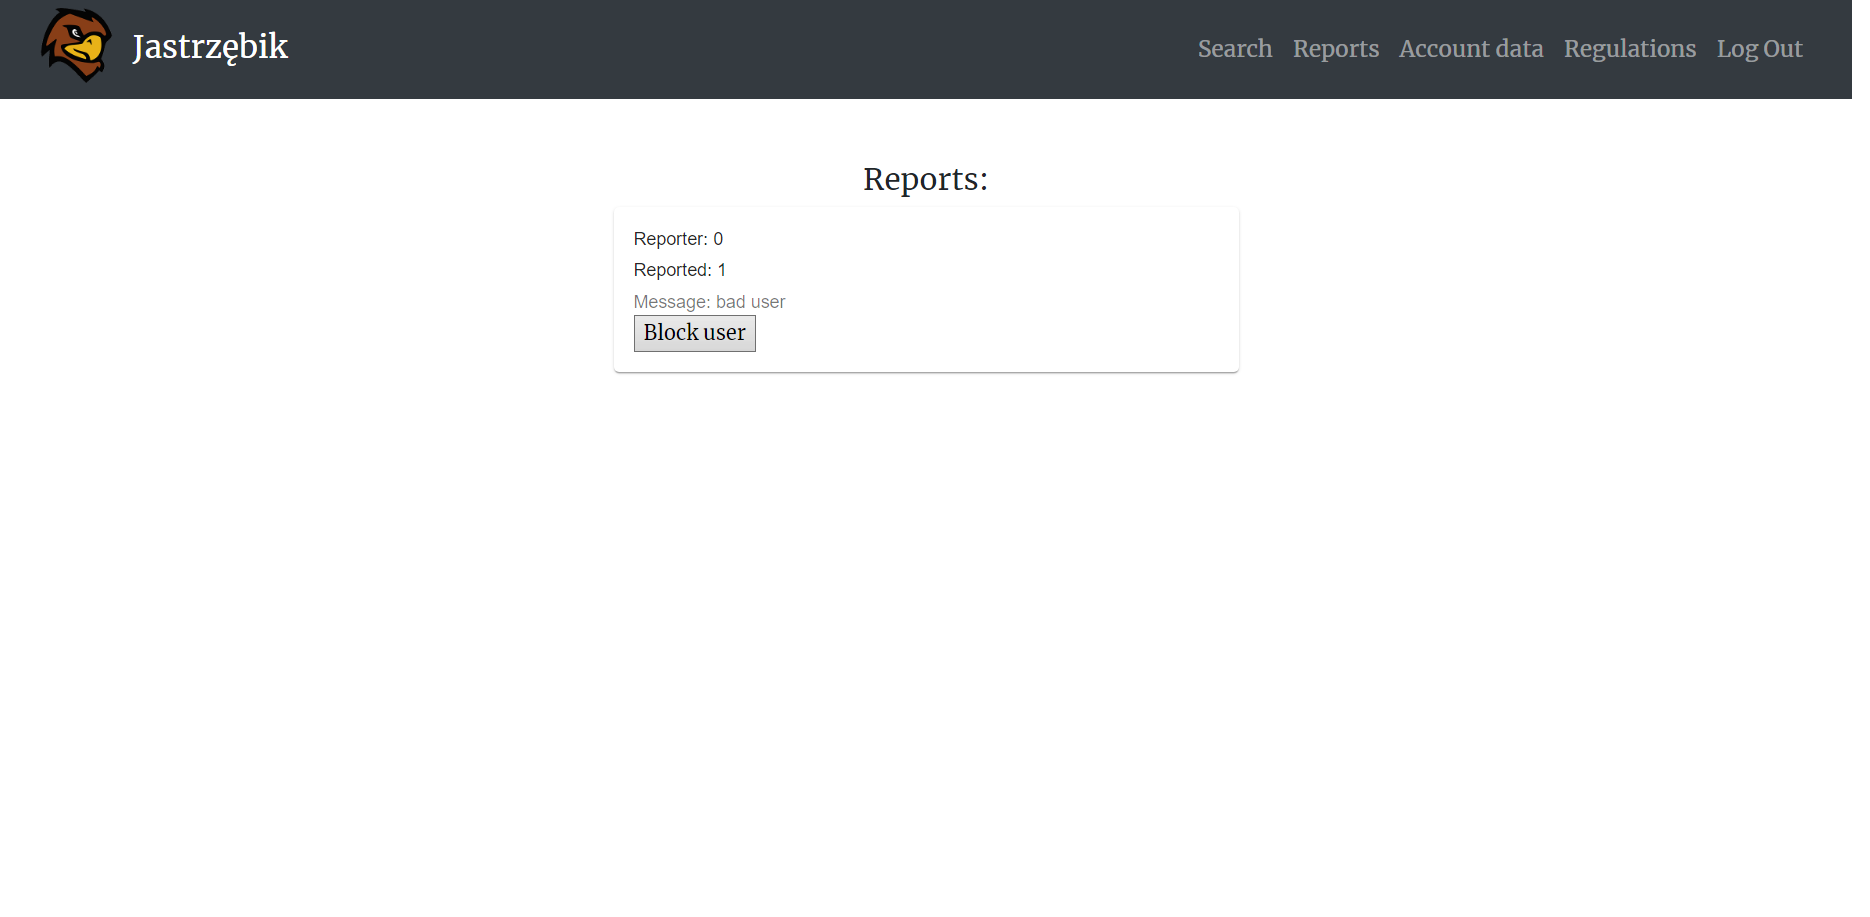
\includegraphics[width=1\textwidth]{img3/Reports.png}
        \caption{Panel z przeglądem zgłoszeń}
        \label{fig:Reports}
    \end{figure}

\end{document}
